\chapter{状態表現の階層性を考慮することによる深層状態空間モデルの拡張}
\label{chap:proposal}

第三章の問題を受け,第四章ではシンプルな帰納バイアスを導入することによってDSSMを拡張する方法を提案する.はじめに本研究で扱う問題設定について改めて整理し,続けて提案手法とその既存の類似手法について述べる.

\section{問題設定の整理}

本研究では行動条件付き映像予測の問題を解く.具体的には,ある行動主体が実行した行動系列$a_{1:10}$と初期観測$o_0$が与えられたときに$o_{1:10}$を生成し,その生成される映像の尤度を高めることを目指す.ただし訓練時には行動系列と観測系列の組$\{\vec{a}, \vec{o}\}$の訓練用のデータセットを用いることができ,評価時には,訓練データには含まれないが訓練データと同じ条件で収集された評価用のデータセットを用いる.
本研究の目的は,この条件付き映像予測問題においてベースラインにDSSMを設定し,DSSMをより複雑な環境での映像予測問題にもスケールできるように拡張することである.

\section{提案手法}
三章で述べたようにベースラインのDSSMでは潜在変数の次元を大きくすると学習がうまくいかなかった.しかし予備実験で得た,低次元の潜在変数を用いたときには部分的に学習が進んだという事実をヒントにし,状態変数の次元を大きくしていく方向性はそのままで状態表現の階層性を考えることにより,より複雑な問題設定においても学習可能なDSSMの拡張方法を提案する.

\begin{figure}[tp]
  \begin{center}
    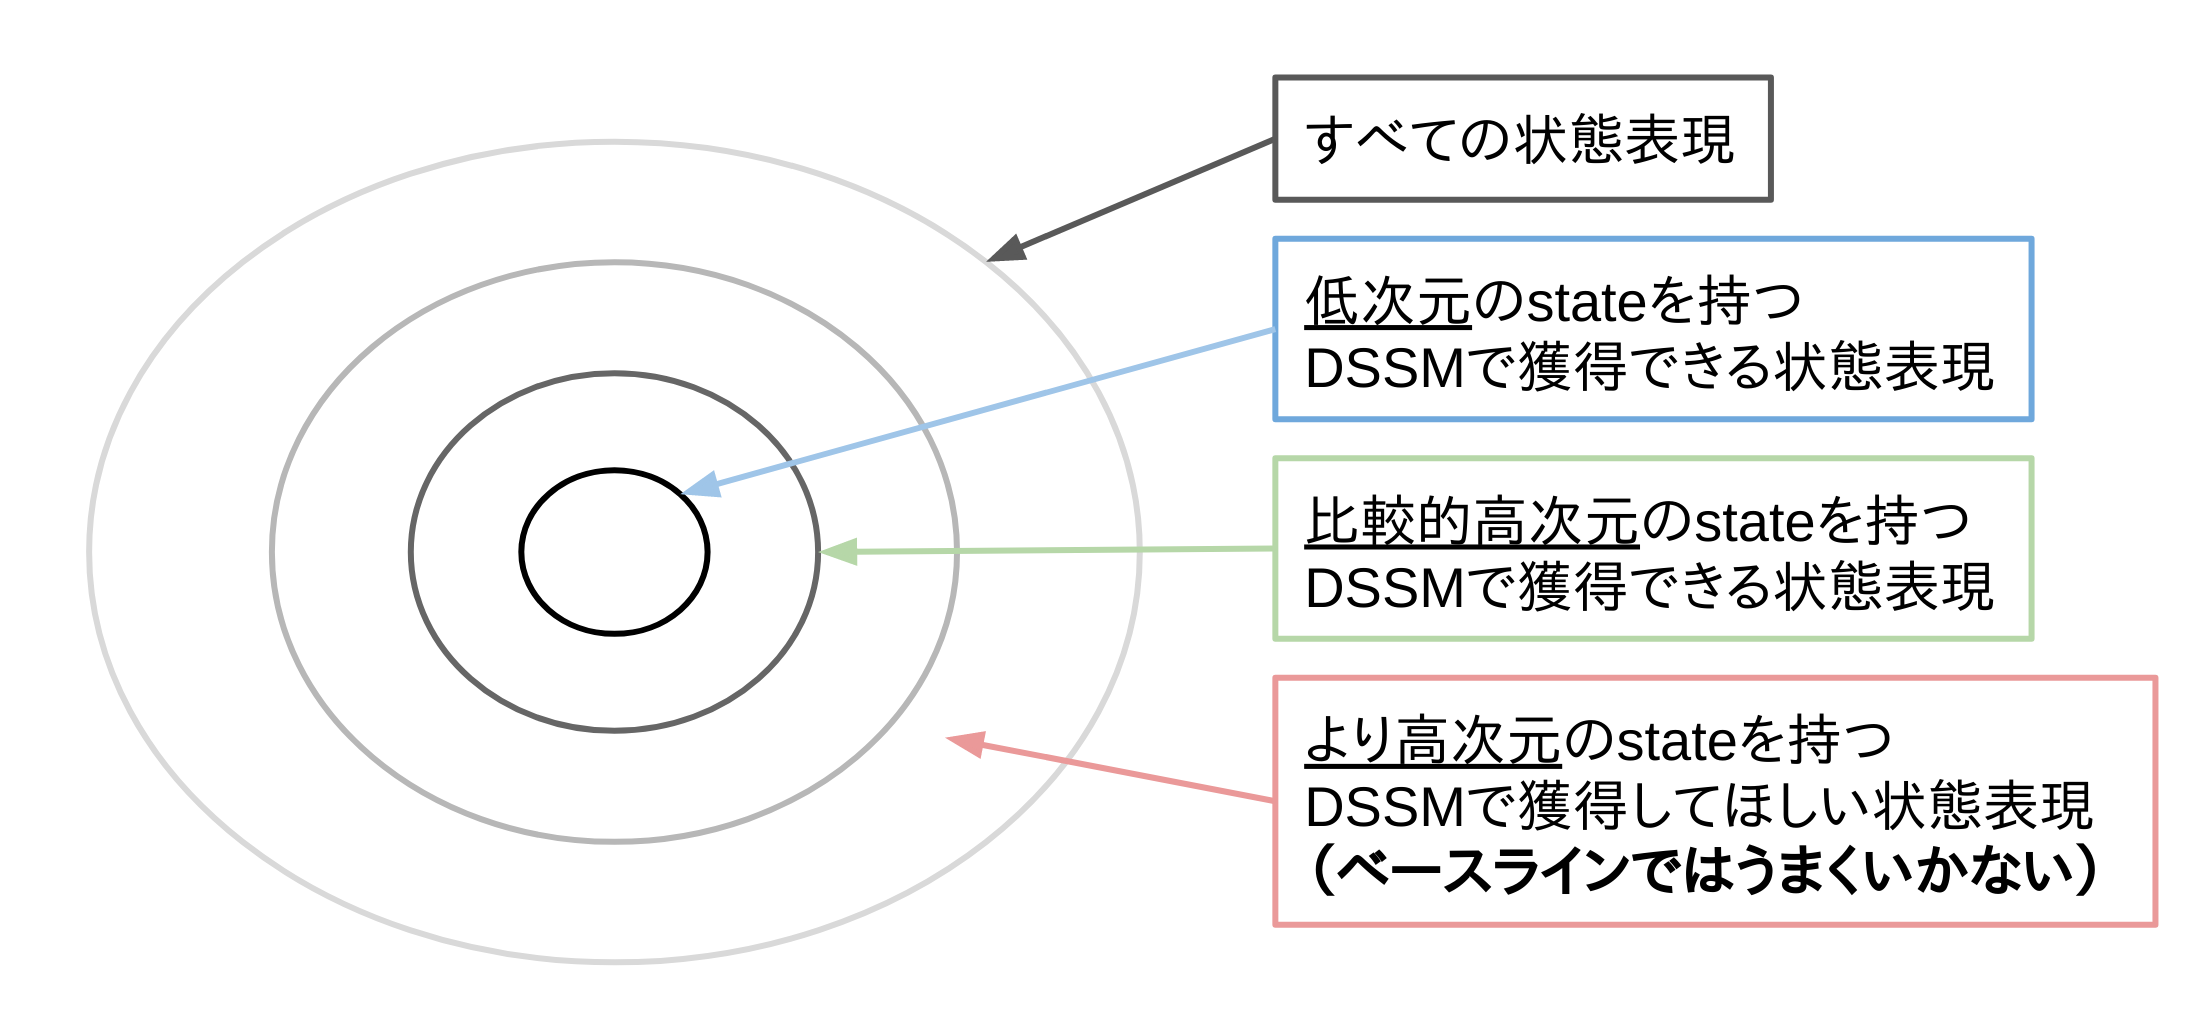
\includegraphics[width=\linewidth]{./figures/hierarchical.png}
    \caption{hierarchical}
    \label{fig:hierarchical}
  \end{center}
\end{figure}

\subsection{状態表現の階層性}
はじめに,ベースラインのDSSMにおいて潜在変数の次元を変えた時に獲得される情報について考察する.低次元の状態変数で獲得できる情報は高次元の状態変数を用いた場合にも当然獲得できると考えた場合,図(\ref{fig:hierarchical})のように高次元の状態変数が持つ情報は低次元の状態変数が持つ情報をほぼ内包していると考えることができる.
ここで状態変数の次元をより大きくしたときに精度がむしろ悪化することが問題であったが,これは三章で述べたとおり,状態変数の次元が大きくなったときに高次元ベクトルから高次元ベクトルへの写像を学習する必要が生じあるべき写像先がなかなか定まらないことが原因であると考えられ,何らかの方法で遷移モデルの学習を補助することで図のようにより多くの情報を獲得できる可能性がある.

\subsection{階層的な状態表現の遷移}
ベースラインの状態表現の遷移は図(\ref{fig:transition_base})が示すように状態変数が持つすべての情報を一度に変換することを考えているが,直感的に一括で変換することは学習が難しいと思われる.状態表現を一括で変換する代わりに,前節のような階層性の概念を導入することで図(\ref{fig:transition_proposal})のように簡単に遷移が学習できる部分から順に遷移させていくような方法を考えることができる.

このような階層的な状態表現の遷移を考えると,はじめから高次元の状態表現の遷移を考えずに学習の習熟度に合わせて徐々に高次元の状態ベクトルの遷移を学習することができ,学習がスムースに進みやすくなると考えられる.

\begin{figure}[tbp]
  \begin{center}
    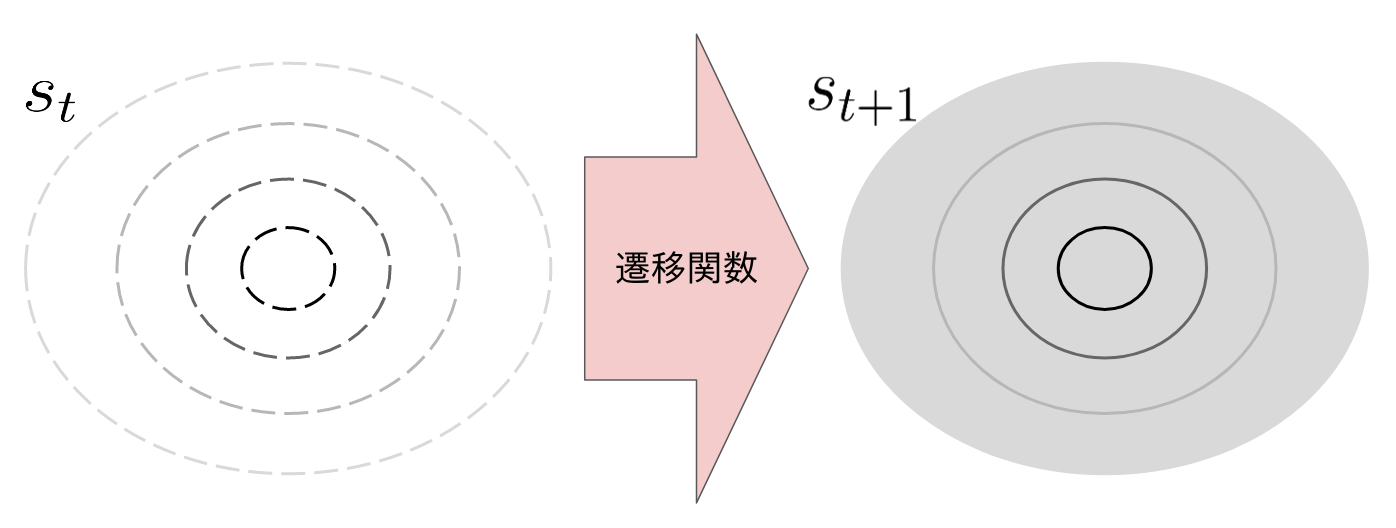
\includegraphics[width=0.5\linewidth]{./figures/transition_base.png}
    \caption{transition base}
    \label{fig:transition_base}
  \end{center}
\end{figure}

\begin{figure}[tbp]
  \begin{center}
    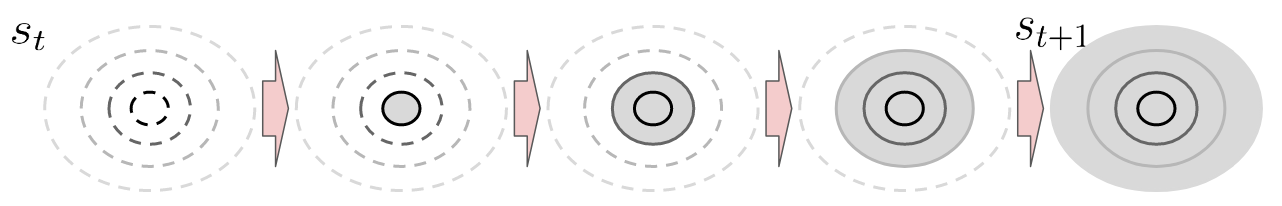
\includegraphics[width=0.8\linewidth]{./figures/transition_proposal.png}
    \caption{transition proposal}
    \label{fig:transition_proposal}
  \end{center}
\end{figure}

% \caption[hoge]{fuga}
\begin{figure}[tbp]
  \begin{center}
    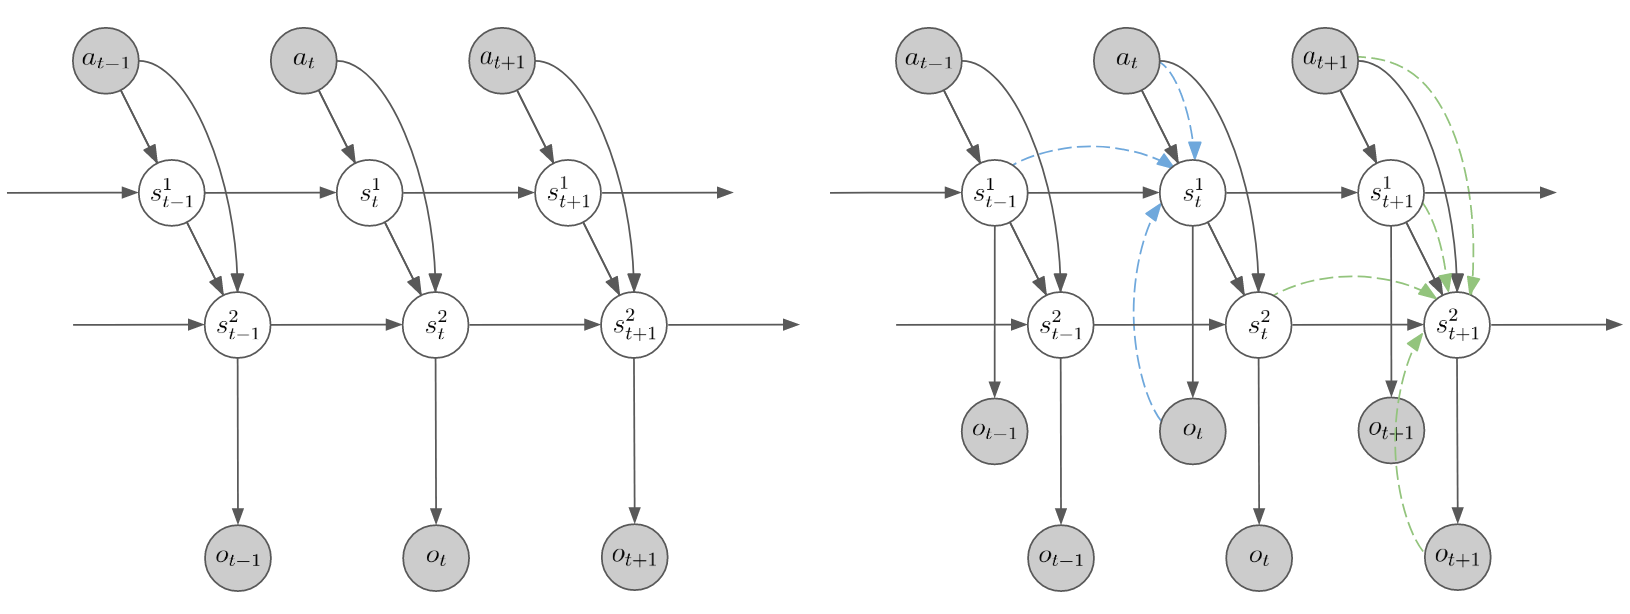
\includegraphics[width=\linewidth]{./figures/proposal.png}
    \caption[提案手法のグラフィカルモデル]{提案手法のグラフィカルモデル.点線の$s^1$, $s^2$の推論分布は簡単のため時刻t, t-1でのみ記載している.proposal (学習時) 2つずつ記載されている$o_t$は同じデータを示すが.異なるsから独立に生成されることを明示している.}
    \label{fig:proposal}
  \end{center}
\end{figure}

\subsection{確率モデル・最適化}

ここまでで状態変数の階層性とその遷移を考えたが,この階層性の仮定はDSSMの性能の向上に十分寄与しうると考え,状態変数の階層性を帰納バイアスとしてDSSMに組み込み以下のようなモデルとその最適化アルゴリズムを提案する.

\vspace{\baselineskip}
提案手法のグラフィカルモデルを図(\ref{fig:proposal})に示す.(TODO: 三層以上の場合も図にする),
提案手法は,DSSMの状態変数をN層に階層化したモデルである.図(\ref{fig:proposal})は2階層の提案モデルを図(\ref{fig:proposal_big} TODO)は3階層以上の提案モデルを表している.図(\ref{fig:proposal})の上側の状態変数から一階層の状態変数・二階層の状態変数と呼ぶことにすると一階層の状態変数が低次元ベクトル,二階層の状態変数が高次元ベクトルになっており,高次元の状態変数の生成・推論時に低次元の状態変数を用いるようなモデルになっている.高次元の状態変数の遷移時に低階層の状態変数を用いて写像先に関する情報を補助的に与えることで,学習を安定化させる効果が期待される.またモデルの評価時には,最高層の観測の生成モデル $p(o_t|s^N_t)$ を用いる.

\begin{algorithm}[tbp]               
  \caption{N階層DSSMの学習アルゴリズム TODO: 書き直す}
  \label{alg1}                          
  \begin{algorithmic}
    \FOR{一階層目からN階層目まで}
      \WHILE{学習が収束していない}
        \STATE 現在の階層より上の階層のパラメータを固定し, 
        \STATE 現在の階層を以下の目的関数で学習する
        \STATE $L(x)$ = その階層での再構成 + その階層の$KL(q||p)$ \\
      \ENDWHILE
    \ENDFOR
  \end{algorithmic}
\end{algorithm}

\vspace{\baselineskip}
次に提案手法の学習アルゴリズムをアルゴリズム\ref{alg1}に示す.この学習アルゴリズムは前節「階層的な状態表現の遷移」で述べた,習熟度に合わせて徐々に高次元の状態ベクトルの遷移を学習するという考え方に基づいており,これにより安定した学習が見込める.今回簡単のために高階層の潜在表現の学習時にはそれより低階層の状態表現の学習を止めているが,他の方法も考えられ,これついては考察「低次元状態ベクトルの階層の再学習」で述べる.



% 確率的生成過程は以下
% \begin{equation}
%   p(o_{1:T}|a_{1:T}) = \prod_{t=1}^T \iint p(o_t|s^2_t) p(s^2_t|s^2_{t-1}, a_t, s^1_t) p(s^1_t|s^1_{t-1}, a_t) d{s^1_t}{ds^2_t}
% \end{equation}


% この時の変分下限は以下
% \begin{eqnarray}
%   \ (ELBO) \nonumber \\
%   &=& \sum_{t=1}^T \left( \mathbb{E}_{s^2_t \sim q(s^2_t|a_{1:t}, o_{1:t})} [\log p(o_t|s^2_t)] \right. \nonumber \\
%   && \hspace{2em} \left. - \mathbb{E}_{s^1_{t-1} \sim q(s^1_{t-1}|a_{1:t-1}, o_{1:t-1}), 改行したい s^2 \sim}  [\mathrm{D_{KL}}(q(s_t|s_{t-1}, a_t, o_t) \| p(s_t|s_{t-1}, a_t, o_t))] \right. \nonumber \\
%   && \hspace{2em} \left. - \mathbb{E}_{s^1_{t-1} \sim q(s^1_{t-1}|a_{1:t-1}, o_{1:t-1}), 改行したい s^2 \sim } [\mathrm{D_{KL}}(q(s_t|s_{t-1}, a_t, o_t) \| p(s_t|s_{t-1}, a_t, o_t))] \right) \nonumber \\
%   \label{eq:hssm_elbo}
% \end{eqnarray}


% 目的関数は以下
% % 
% \begin{eqnarray}
%   \ (目的関数) \nonumber \\
%   &=& \sum_{t=1}^T \left( \mathbb{E}_{s^2_t \sim q(s^2_t|a_{1:t}, o_{1:t})} [\log p(o_t|s^2_t)] + \beta \mathbb{E}_{s^1_t \sim q(s^1_t|a_{1:t}, o_{1:t})} [\log p(o_t|s^1_t)] \right. \nonumber \\
%   && \hspace{2em} \left. - \mathbb{E}_{s^1_{t-1} \sim q(s^1_{t-1}|a_{1:t-1}, o_{1:t-1}), 改行したい s^2 \sim}  [\mathrm{D_{KL}}(q(s_t|s_{t-1}, a_t, o_t) \| p(s_t|s_{t-1}, a_t, o_t))] \right. \nonumber \\
%   && \hspace{2em} \left. - \mathbb{E}_{s^1_{t-1} \sim q(s^1_{t-1}|a_{1:t-1}, o_{1:t-1}), 改行したい s^2 \sim } [\mathrm{D_{KL}}(q(s_t|s_{t-1}, a_t, o_t) \| p(s_t|s_{t-1}, a_t, o_t))] \right) \nonumber \\
%   \label{eq:hssm_loss}
% \end{eqnarray}

\section{類似手法との差分 TODO}
提案手法と類似手法の差分について整理する.DSSM自体を用いた映像予測の研究はこれまであまりされていないが,これは1章でも述べたとおりDSSMは自己回帰モデルと比べて高精度な生成には向いていないためだと考えられる.そのため本節では階層性を考慮した画像生成と映像生成の既存研究について取り上げる.

まずモデルに階層性を取り入れた画像生成の先行研究としてDRAW[引用],PGGAN[引用]があり,映像予測で階層的なモデルを扱う手法としFutureGAN[引用],てVRNN[引用]がある.DRAWはVAEベースの深層生成モデルであり,潜在変数を複数用意し階層的にすることでデータの潜在表現に単純な正規分布を仮定しないより複雑な表現を可能にしている.提案手法はDRAWを時間変化するデータを扱う問題設定に拡張したようなモデルとなっているが,DRAWは一度にすべての潜在表現を学習するのに対し,時系列データを扱う提案手法では毎時刻の状態表現の遷移を学習することが難しいため潜在表現を順に学習するアルゴリズムを採用している.PGGANは敵対的生成モデルを用いた画像生成手法で,低解像度の画像の生成からはじめ,学習が進むにつれてニューラルネットワークモデルを徐々に多層にすることで高解像度の画像生成を行う.低次元の隠れ変数を変数から学習していくという点で提案手法と似ているが,PGGANは何も条件付けしない生成を行っており,過去の状態や行動で条件付けして画像を生成する行動条件付き映像予測の問題設定に用いる方法は自明ではなかった.FutureGANはPGGANを映像予測に応用した手法で,過去の6フレーム程度の映像を入力とし未来の25フレーム程度の映像を予測することができる.VRNNは直前のフレームを用いて次のフレームを予測する自己回帰モデルになっており,潜在変数から画像を出力する過程で得られる隠れ変数を次の時刻の画像の出力にも用いるようにして潜在変数の階層性を考えたモデルになっている.FutureGANやVRNNは予測する際に過去数フレームの映像を用意する必要があるが,ベースラインのDSSMや提案手法では初期状態の推論用に過去1フレームだけを用いれば良いモデルになっている.

RNNやLSTMを用いた自己回帰モデルになっており,
\begin{itemize}
  \item DRAW[]はVAEの潜在変数に階層性をもたせたモデル画像生成で用いられる
  \item 多層RNN[]は
  \item PGANは平面状の隠れ変数の次元を徐々に大きくすることで徐々に高解像度の映像生成を可能にする敵対的生成ネットワークベース手法で,
  \item FutureGANは,6フレームの映像を入力としてその後に続く30フレームを予測するような問題設定を解くGANベースの手法で,潜在変数を徐々にある.こちらは入力として複数フレーム与えられるので本研究の
  また,確率的な遷移を考えていない.
\end{itemize}

表:必要な入力フレーム数,条件付け,映像か画像か

% あれaction conditionlな先行研究って,visual forsightとか,SV2Pとかしかなかったっけ?

% videoflowはaction conditionalじゃないしー

